\documentclass[]{book}
\usepackage{lmodern}
\usepackage{amssymb,amsmath}
\usepackage{ifxetex,ifluatex}
\usepackage{fixltx2e} % provides \textsubscript
\ifnum 0\ifxetex 1\fi\ifluatex 1\fi=0 % if pdftex
  \usepackage[T1]{fontenc}
  \usepackage[utf8]{inputenc}
\else % if luatex or xelatex
  \ifxetex
    \usepackage{mathspec}
  \else
    \usepackage{fontspec}
  \fi
  \defaultfontfeatures{Ligatures=TeX,Scale=MatchLowercase}
\fi
% use upquote if available, for straight quotes in verbatim environments
\IfFileExists{upquote.sty}{\usepackage{upquote}}{}
% use microtype if available
\IfFileExists{microtype.sty}{%
\usepackage{microtype}
\UseMicrotypeSet[protrusion]{basicmath} % disable protrusion for tt fonts
}{}
\usepackage[margin=1in]{geometry}
\usepackage{hyperref}
\hypersetup{unicode=true,
            pdftitle={Course Notes for Social Networking},
            pdfauthor={Zack W. Almquist},
            pdfborder={0 0 0},
            breaklinks=true}
\urlstyle{same}  % don't use monospace font for urls
\usepackage{natbib}
\bibliographystyle{apalike}
\usepackage{color}
\usepackage{fancyvrb}
\newcommand{\VerbBar}{|}
\newcommand{\VERB}{\Verb[commandchars=\\\{\}]}
\DefineVerbatimEnvironment{Highlighting}{Verbatim}{commandchars=\\\{\}}
% Add ',fontsize=\small' for more characters per line
\usepackage{framed}
\definecolor{shadecolor}{RGB}{248,248,248}
\newenvironment{Shaded}{\begin{snugshade}}{\end{snugshade}}
\newcommand{\KeywordTok}[1]{\textcolor[rgb]{0.13,0.29,0.53}{\textbf{{#1}}}}
\newcommand{\DataTypeTok}[1]{\textcolor[rgb]{0.13,0.29,0.53}{{#1}}}
\newcommand{\DecValTok}[1]{\textcolor[rgb]{0.00,0.00,0.81}{{#1}}}
\newcommand{\BaseNTok}[1]{\textcolor[rgb]{0.00,0.00,0.81}{{#1}}}
\newcommand{\FloatTok}[1]{\textcolor[rgb]{0.00,0.00,0.81}{{#1}}}
\newcommand{\ConstantTok}[1]{\textcolor[rgb]{0.00,0.00,0.00}{{#1}}}
\newcommand{\CharTok}[1]{\textcolor[rgb]{0.31,0.60,0.02}{{#1}}}
\newcommand{\SpecialCharTok}[1]{\textcolor[rgb]{0.00,0.00,0.00}{{#1}}}
\newcommand{\StringTok}[1]{\textcolor[rgb]{0.31,0.60,0.02}{{#1}}}
\newcommand{\VerbatimStringTok}[1]{\textcolor[rgb]{0.31,0.60,0.02}{{#1}}}
\newcommand{\SpecialStringTok}[1]{\textcolor[rgb]{0.31,0.60,0.02}{{#1}}}
\newcommand{\ImportTok}[1]{{#1}}
\newcommand{\CommentTok}[1]{\textcolor[rgb]{0.56,0.35,0.01}{\textit{{#1}}}}
\newcommand{\DocumentationTok}[1]{\textcolor[rgb]{0.56,0.35,0.01}{\textbf{\textit{{#1}}}}}
\newcommand{\AnnotationTok}[1]{\textcolor[rgb]{0.56,0.35,0.01}{\textbf{\textit{{#1}}}}}
\newcommand{\CommentVarTok}[1]{\textcolor[rgb]{0.56,0.35,0.01}{\textbf{\textit{{#1}}}}}
\newcommand{\OtherTok}[1]{\textcolor[rgb]{0.56,0.35,0.01}{{#1}}}
\newcommand{\FunctionTok}[1]{\textcolor[rgb]{0.00,0.00,0.00}{{#1}}}
\newcommand{\VariableTok}[1]{\textcolor[rgb]{0.00,0.00,0.00}{{#1}}}
\newcommand{\ControlFlowTok}[1]{\textcolor[rgb]{0.13,0.29,0.53}{\textbf{{#1}}}}
\newcommand{\OperatorTok}[1]{\textcolor[rgb]{0.81,0.36,0.00}{\textbf{{#1}}}}
\newcommand{\BuiltInTok}[1]{{#1}}
\newcommand{\ExtensionTok}[1]{{#1}}
\newcommand{\PreprocessorTok}[1]{\textcolor[rgb]{0.56,0.35,0.01}{\textit{{#1}}}}
\newcommand{\AttributeTok}[1]{\textcolor[rgb]{0.77,0.63,0.00}{{#1}}}
\newcommand{\RegionMarkerTok}[1]{{#1}}
\newcommand{\InformationTok}[1]{\textcolor[rgb]{0.56,0.35,0.01}{\textbf{\textit{{#1}}}}}
\newcommand{\WarningTok}[1]{\textcolor[rgb]{0.56,0.35,0.01}{\textbf{\textit{{#1}}}}}
\newcommand{\AlertTok}[1]{\textcolor[rgb]{0.94,0.16,0.16}{{#1}}}
\newcommand{\ErrorTok}[1]{\textcolor[rgb]{0.64,0.00,0.00}{\textbf{{#1}}}}
\newcommand{\NormalTok}[1]{{#1}}
\usepackage{longtable,booktabs}
\usepackage{graphicx,grffile}
\makeatletter
\def\maxwidth{\ifdim\Gin@nat@width>\linewidth\linewidth\else\Gin@nat@width\fi}
\def\maxheight{\ifdim\Gin@nat@height>\textheight\textheight\else\Gin@nat@height\fi}
\makeatother
% Scale images if necessary, so that they will not overflow the page
% margins by default, and it is still possible to overwrite the defaults
% using explicit options in \includegraphics[width, height, ...]{}
\setkeys{Gin}{width=\maxwidth,height=\maxheight,keepaspectratio}
\IfFileExists{parskip.sty}{%
\usepackage{parskip}
}{% else
\setlength{\parindent}{0pt}
\setlength{\parskip}{6pt plus 2pt minus 1pt}
}
\setlength{\emergencystretch}{3em}  % prevent overfull lines
\providecommand{\tightlist}{%
  \setlength{\itemsep}{0pt}\setlength{\parskip}{0pt}}
\setcounter{secnumdepth}{5}
% Redefines (sub)paragraphs to behave more like sections
\ifx\paragraph\undefined\else
\let\oldparagraph\paragraph
\renewcommand{\paragraph}[1]{\oldparagraph{#1}\mbox{}}
\fi
\ifx\subparagraph\undefined\else
\let\oldsubparagraph\subparagraph
\renewcommand{\subparagraph}[1]{\oldsubparagraph{#1}\mbox{}}
\fi

%%% Use protect on footnotes to avoid problems with footnotes in titles
\let\rmarkdownfootnote\footnote%
\def\footnote{\protect\rmarkdownfootnote}

%%% Change title format to be more compact
\usepackage{titling}

% Create subtitle command for use in maketitle
\newcommand{\subtitle}[1]{
  \posttitle{
    \begin{center}\large#1\end{center}
    }
}

\setlength{\droptitle}{-2em}
  \title{Course Notes for Social Networking}
  \pretitle{\vspace{\droptitle}\centering\huge}
  \posttitle{\par}
  \author{Zack W. Almquist}
  \preauthor{\centering\large\emph}
  \postauthor{\par}
  \predate{\centering\large\emph}
  \postdate{\par}
  \date{2017-12-29}

\usepackage{booktabs}
\usepackage{amsthm}
\makeatletter
\def\thm@space@setup{%
  \thm@preskip=8pt plus 2pt minus 4pt
  \thm@postskip=\thm@preskip
}
\makeatother

\usepackage{amsthm}
\newtheorem{theorem}{Theorem}[chapter]
\newtheorem{lemma}{Lemma}[chapter]
\theoremstyle{definition}
\newtheorem{definition}{Definition}[chapter]
\newtheorem{corollary}{Corollary}[chapter]
\newtheorem{proposition}{Proposition}[chapter]
\theoremstyle{definition}
\newtheorem{example}{Example}[chapter]
\theoremstyle{definition}
\newtheorem{exercise}{Exercise}[chapter]
\theoremstyle{remark}
\newtheorem*{remark}{Remark}
\newtheorem*{solution}{Solution}
\let\BeginKnitrBlock\begin \let\EndKnitrBlock\end
\begin{document}
\maketitle

{
\setcounter{tocdepth}{1}
\tableofcontents
}
\chapter{Prerequisites}\label{prerequisites}

This is a set of \emph{course notes} for SOCIOLOGY 3412: Social
Networking. All examples are written in the
\href{https://www.r-project.org/}{R} Statistical programing language. It
is recommended that you use \href{https://www.rstudio.com/}{R-Studio} as
your
\href{https://en.wikipedia.org/wiki/Integrated_development_environment}{IDE}
for this course as it is the one that will be demonstrated in lecture.

\section{R}\label{r}

R is a statistical programming language that is popular in industry and
acadamia. It is open source and has very powerful tools for analysis and
visualization. I recommend running yourself through an online tutorial
before the course begins. A popular one is run by \emph{DataCamp} and is
free and can be found
\href{https://www.datacamp.com/courses/free-introduction-to-r}{here}.
However, there are a number of alternatives, all of which can be found
on \href{http://www.letmegooglethat.com/?q=introduction+to+R}{google}.

\section{STATNET and igraph}\label{statnet-and-igraph}

We will be using the following packages from the
\href{https://statnet.org/}{STATNET} project:

\begin{Shaded}
\begin{Highlighting}[]
\KeywordTok{install.packages}\NormalTok{(}\StringTok{'network'}\NormalTok{)}
\KeywordTok{install.packages}\NormalTok{(}\StringTok{'ergm'}\NormalTok{)}
\KeywordTok{install.packages}\NormalTok{(}\StringTok{'sna'}\NormalTok{)}
\KeywordTok{install.packages}\NormalTok{(}\StringTok{'EpiModel)}
\end{Highlighting}
\end{Shaded}

We will also on occasion make use of the \textbf{igraph} package:

\begin{Shaded}
\begin{Highlighting}[]
\KeywordTok{install.packages}\NormalTok{(}\StringTok{'igraph'}\NormalTok{)}
\end{Highlighting}
\end{Shaded}

\section{networkdata and devtools}\label{networkdata-and-devtools}

We will occasionally use packages created by the author and installed
via \href{github.com/}{github}. To do this you will first need to
install \textbf{devtools}:

\begin{Shaded}
\begin{Highlighting}[]
\KeywordTok{install.packages}\NormalTok{(}\StringTok{"devtools"}\NormalTok{)}
\end{Highlighting}
\end{Shaded}

Then you can install the \textbf{networkdata} package and other packages
created for this course as needed, e.g.,

\begin{Shaded}
\begin{Highlighting}[]
\KeywordTok{library}\NormalTok{(devtools)}
\KeywordTok{install_github}\NormalTok{(}\StringTok{"zalmquist/networkdata"}\NormalTok{)}
\end{Highlighting}
\end{Shaded}

\chapter{Networks and Network Thinking}\label{IntroNetworks}

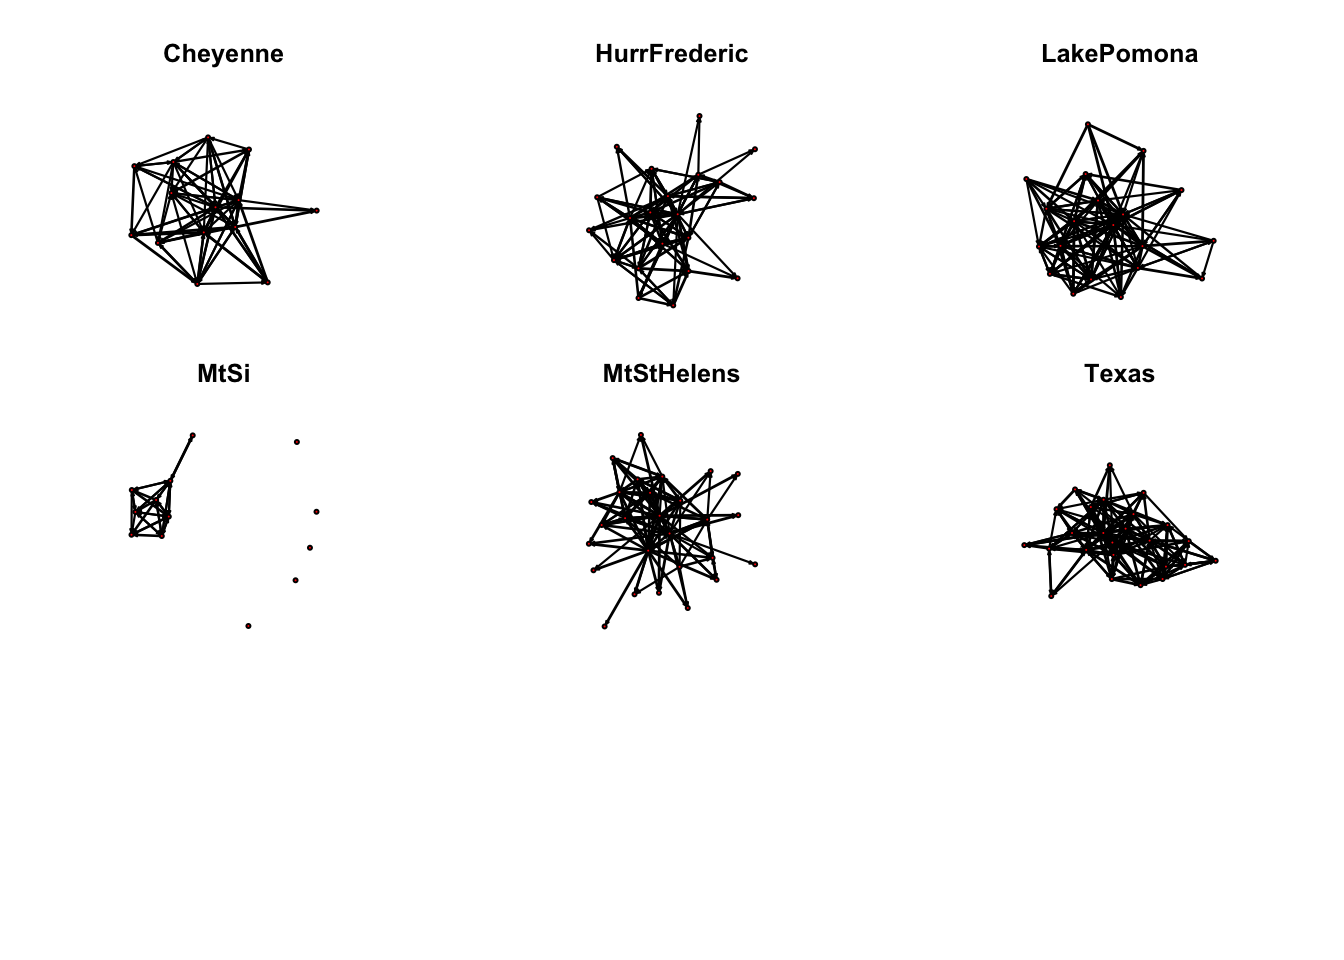
\includegraphics{IntroToNetworks_files/figure-latex/unnamed-chunk-6-1.pdf}

\section{Overview}\label{overview}

Network science and social network analysis provide both a theoretical
and methodological foundation for understanding our social world.
\citet{butts08} explains the social network field as follows:

\begin{quote}
The social network field is an interdisciplinary research program which
seeks to predict the structure of relation- ships among social entities,
as well as the impact of said structure on other social phenomena. The
substantive elements of this program are built around a shared chore of
concepts and methods for the measurement, representation, and analysis
of social structure. These techniques (jointly referred to as the
methods of social network analysis) are applicable to a wide range of
substantive domains, ranging from the analysis of concepts within mental
models (\citet{wegner95},\citet{carley97}) to the study of war between
nations (\citet{wimmer06})
\end{quote}

\section{Introduction to Network
Concepts}\label{introduction-to-network-concepts}

To begin our journey into the nature of social networks, we first must
define what a \textbf{relationship} entails.

\BeginKnitrBlock{definition}
\protect\hypertarget{def:unnamed-chunk-7}{}{\label{def:unnamed-chunk-7}
}\emph{Relationship}: an irreducible property of two or more entities
(compare with properties of entities alone or so called ``attributes'').
\EndKnitrBlock{definition}

\BeginKnitrBlock{example}
\protect\hypertarget{exm:unnamed-chunk-8}{}{\label{exm:unnamed-chunk-8} }An
example of a relationship is students alma matters. I.e. Bill graduated
from the University of California, Irvine and Jane graduated from
University of California, Irvine so they have a this ``alma matter''
relationship; however, Bob graduated from University of Michigan so he
is not have this ``alma matter'' relationship with Bill and Jane.

Other examples of relationships can be communication, acquaintanceship,
sexual contact, proximity, migration rate, alliance/conflict, etc.
\EndKnitrBlock{example}

\emph{Focus}: the properties and consequences of relations (rather than
individual properties) * Entities can be persons, non-human animals,
groups, locations, organizations, regions, etc. * Relationships can be
communication, acquaintanceship, sexual contact, proximity, migration
rates, alliance/conflict, etc. * Social network analysis: the study of
relational data arising from social systems

\BeginKnitrBlock{definition}
\protect\hypertarget{def:unnamed-chunk-9}{}{\label{def:unnamed-chunk-9}
}\textbf{Social network analysis}: the study of relational data arising
from social systems (e.g., schools, prisons, countries,\ldots{}).
\EndKnitrBlock{definition}

\BeginKnitrBlock{definition}
\protect\hypertarget{def:unnamed-chunk-10}{}{\label{def:unnamed-chunk-10}
}\textbf{Network}: a collection of entities (commonly called nodes or
vertices), together with a set of relations on those entities (often
called edges or ties).

\begin{enumerate}
\def\labelenumi{\arabic{enumi})}
\tightlist
\item
  Entities: nodes, or vertices
\item
  Relations: edges, or ties (sometimes authors will distinguish between
  tie and edge, however this is somewhat uncommon)
\end{enumerate}

\begin{itemize}
\tightlist
\item
  Focus on dyadic relations
\item
  Directed vs.~undirected
\item
  May be signed or valued

  \EndKnitrBlock{definition}
\end{itemize}

\BeginKnitrBlock{definition}
\protect\hypertarget{def:unnamed-chunk-11}{}{\label{def:unnamed-chunk-11}
}\textbf{Graph}: a set of vertices (\(V\)) together with a set of edges
(\(E\)) -- mathematical representation of social structure. Typically a
graph, \(G\), is define as the set, \(G=(V,E)\)

Below is R code for generating a dyad and ploting it. The vertex set
coorisponds to the number of rows/columns and the edges (relationships)
to the cells in the matrix. More on this in the next section.
\EndKnitrBlock{definition}

\begin{Shaded}
\begin{Highlighting}[]
\KeywordTok{library}\NormalTok{(sna)}
\NormalTok{g<-}\KeywordTok{matrix}\NormalTok{(}\DecValTok{1}\NormalTok{,}\DataTypeTok{nc=}\DecValTok{2}\NormalTok{,}\DataTypeTok{nr=}\DecValTok{2}\NormalTok{)}
\KeywordTok{gplot}\NormalTok{(g)}
\end{Highlighting}
\end{Shaded}

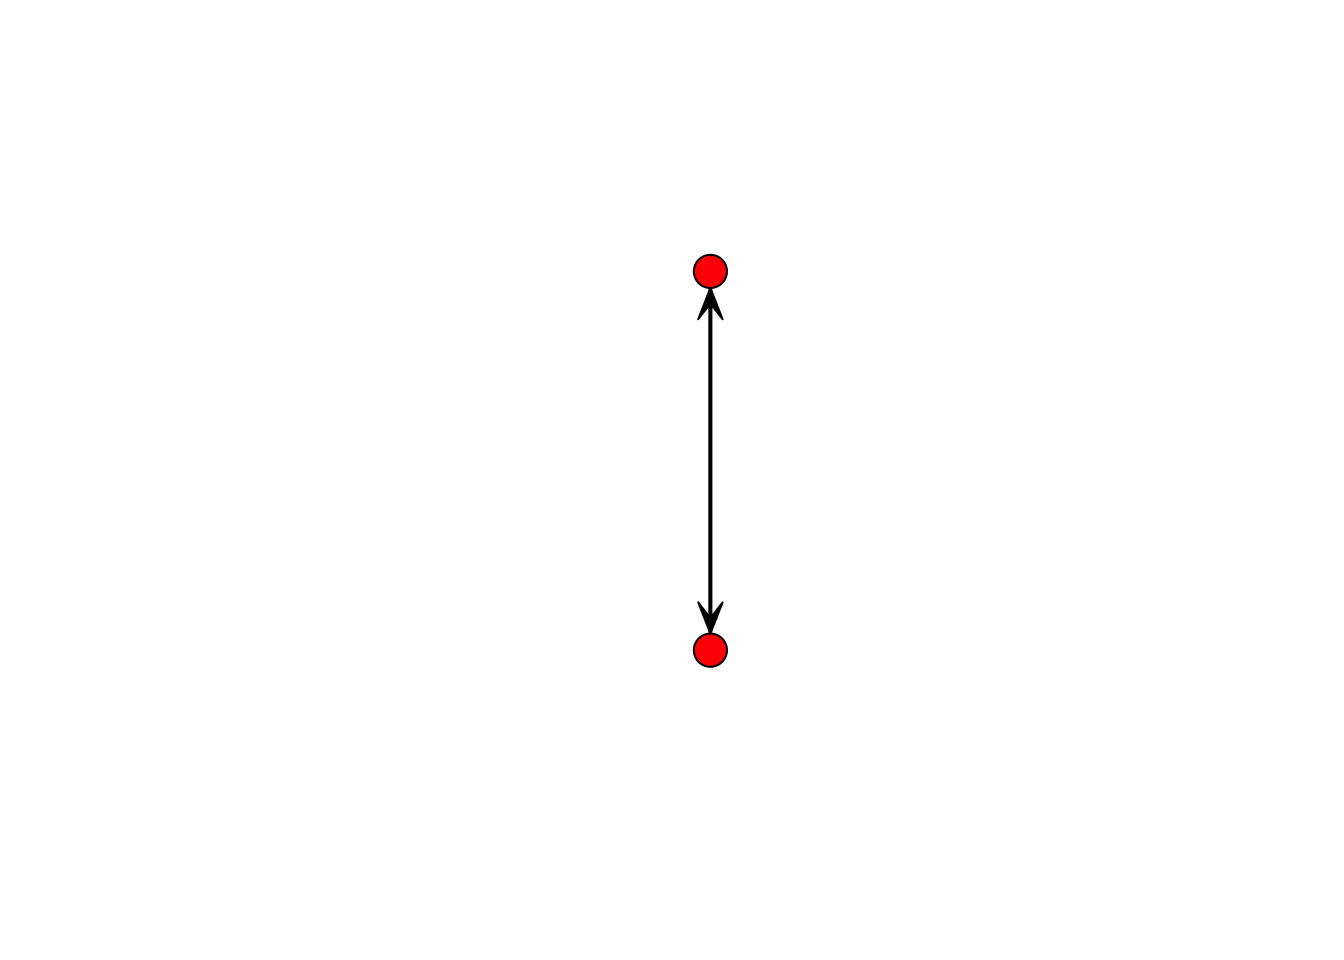
\includegraphics{IntroToNetworks_files/figure-latex/unnamed-chunk-12-1.pdf}

\subsection{Set theoretic notation versus Matrix
Notation}\label{set-theoretic-notation-versus-matrix-notation}

A nework is often represented as a mathematical graph (\(G\)), such that
\(V= \{v_1,\dots,v_n\}\) and \(E\) is the set of \(i,j\) vertices that
have a relation. \(i,j\) can be ordered \((i,j)\) or unordered
\(\{i,j\}\). Ordered ties represent directed relations (e.g., sending a
package) and unordered represent a recipricol relation (e.g., a facebook
friendship). Alternatively, graphs can be represented simply as a square
\textbf{matrix} of binary values (i.e., does a relation exist between
\(i,j\) vertices?). This matrix is known as an adjacency matrix (\(A\)).
An adjancy matrix is binary in the cells (i.e., 1 or 0), typically we
exclude self ties (i.e., \(i,i\) cells are 0) and is always square. If
it is not symmetic then it is a \emph{directed} graph, and if it is
symmetric it is known as \emph{undirected} graph.

Let's visualize an adjancy matrix in R.

\begin{Shaded}
\begin{Highlighting}[]
\NormalTok{g<-}\KeywordTok{rgraph}\NormalTok{(}\DecValTok{10}\NormalTok{)}
\NormalTok{g}
\end{Highlighting}
\end{Shaded}

\section{Relational Data}\label{relational-data}

\BeginKnitrBlock{definition}
\protect\hypertarget{def:unnamed-chunk-14}{}{\label{def:unnamed-chunk-14}
}\textbf{Relational} (network) data\} concerns connections among
entities, rather than attributes of entities * Entities can be persons,
organizations, concepts, etc. * Relations can be interaction, proximity,
membership, etc. * Two common forms of data are \emph{one-mode} data
(adjacency matrices) and \emph{two-mode} data (incidence matrices)
\EndKnitrBlock{definition}

\BeginKnitrBlock{definition}
\protect\hypertarget{def:unnamed-chunk-15}{}{\label{def:unnamed-chunk-15}
}\emph{One Mode data} -- Networks with one vertex class (ie
organizations, individuals, concepts, etc.)

Represented by adjacency matrices. Vertices on rows and columns,
\(A_{ij}=1\) if i sends a tie to j, else \(A_{ij}=0\). Can contain edge
values, where applicable (\(A_{ij}\) is value of i,j edge). Symmetric in
undirected case, diagonals represent self-ties, often treated as
undefined.
\EndKnitrBlock{definition}

\BeginKnitrBlock{example}
\protect\hypertarget{exm:unnamed-chunk-16}{}{\label{exm:unnamed-chunk-16}
}The first example is a communication Emergent A communication network
of the Emergent Multi-Organizational Network (EMON) of Mt Si SAR, data
contained within the network package.
\EndKnitrBlock{example}

R code:

\begin{Shaded}
\begin{Highlighting}[]
\KeywordTok{library}\NormalTok{(network)}
\KeywordTok{data}\NormalTok{(emon)}
\CommentTok{#help(emon)}
 \NormalTok{n <-}\StringTok{ }\KeywordTok{ncol}\NormalTok{(}\KeywordTok{as.sociomatrix}\NormalTok{(emon[[}\DecValTok{4}\NormalTok{]]))}
 \NormalTok{colorn <-}\StringTok{ }\KeywordTok{rainbow}\NormalTok{(n, }\DataTypeTok{start=}\NormalTok{.}\DecValTok{7}\NormalTok{, }\DataTypeTok{end=}\NormalTok{.}\DecValTok{1}\NormalTok{)}
 \NormalTok{vname <-}\StringTok{ }\KeywordTok{get.vertex.attribute}\NormalTok{(emon[[}\DecValTok{4}\NormalTok{]],}\DataTypeTok{attrname=}\StringTok{"vertex.names"}\NormalTok{)}
 \KeywordTok{plot.network}\NormalTok{(emon[[}\DecValTok{4}\NormalTok{]], }\DataTypeTok{usearrows=}\OtherTok{FALSE}\NormalTok{, }\DataTypeTok{displayisolates=}\OtherTok{FALSE}\NormalTok{,}\DataTypeTok{vertex.col=}\NormalTok{colorn,}\DataTypeTok{main=}\StringTok{"Mt. Si SAR EMON"}\NormalTok{)}
\KeywordTok{legend}\NormalTok{(}\StringTok{"topleft"}\NormalTok{,}\DataTypeTok{legend=}\NormalTok{vname, }\DataTypeTok{col=}\NormalTok{colorn, }\DataTypeTok{pch=}\DecValTok{19}\NormalTok{,}\DataTypeTok{bty=}\StringTok{"n"}\NormalTok{,}\DataTypeTok{cex=}\NormalTok{.}\DecValTok{5}\NormalTok{)}
\end{Highlighting}
\end{Shaded}

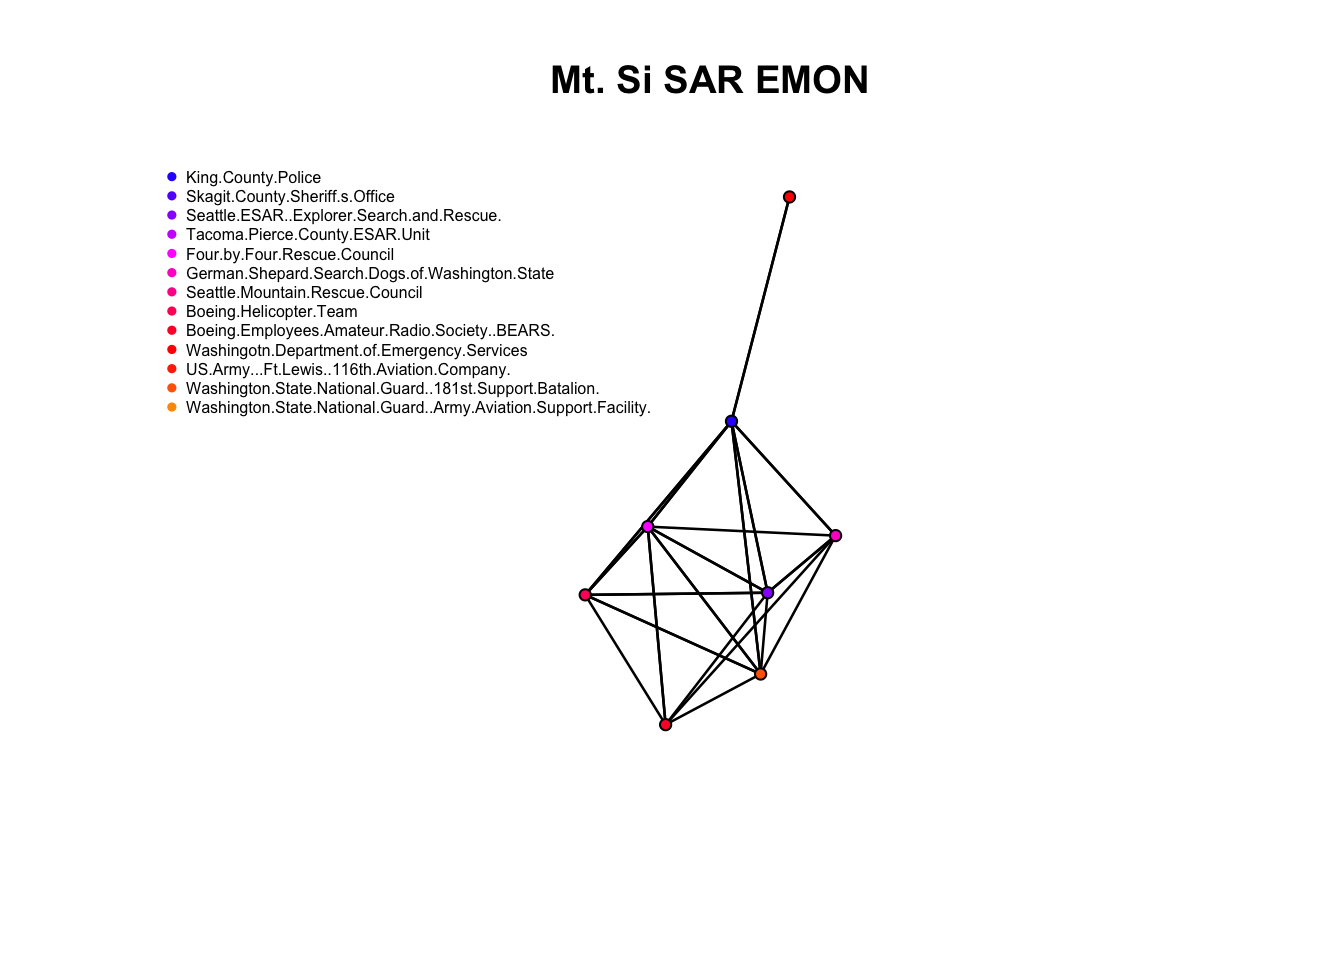
\includegraphics{IntroToNetworks_files/figure-latex/unnamed-chunk-17-1.pdf}

Edge list a,b; c,d; e,f; etc incident matrices

\BeginKnitrBlock{example}
\protect\hypertarget{exm:unnamed-chunk-18}{}{\label{exm:unnamed-chunk-18}
}Special Case: Ego Nets-- Egocentric network: focal actor (``ego'') and
neighbors (``alters'') and ties among alters. What does it tell us:
number of ties ego has (neighborhood size), Triangles (3-cliques)
containing ego, connections among alters, neighborhood composition (if
asked) \%find an example graph it and put it here
\EndKnitrBlock{example}

\subsection{Some Types of
Relationships}\label{some-types-of-relationships}

\begin{itemize}
\tightlist
\item
  Conceptual: shared or antithetic properties

  \begin{itemize}
  \tightlist
  \item
    similarity/difference in individual attributes, correlation among
    variables, inclusion/exclusion, surface matching on proteins
  \end{itemize}
\item
  Co-catagorical: shared membership

  \begin{itemize}
  \tightlist
  \item
    organizational co-membership, event co-participation, co-occurrence
    of words within texts
  \end{itemize}
\item
  Nominational: resulting from the behavior of ego +attributions of
  friendship/enmity, kinship (fictive or otherwise), causal narratives
\end{itemize}

\BeginKnitrBlock{example}
\protect\hypertarget{exm:unnamed-chunk-19}{}{\label{exm:unnamed-chunk-19} }
* Macro-level networks +include: militarized interstate disputes,
migration networks (e.g.~county-couty migration in the US),
interorganizational relations (e.g.~SAR EMONs)
\EndKnitrBlock{example}

R code

\begin{Shaded}
\begin{Highlighting}[]
\KeywordTok{load}\NormalTok{(}\StringTok{"data/cow_adjmats.Rdata"}\NormalTok{)}
\NormalTok{mid.network<-}\KeywordTok{as.network}\NormalTok{(mid[[}\DecValTok{1}\NormalTok{]])}
\KeywordTok{plot.network}\NormalTok{(mid.network,}\DataTypeTok{displayisolates=}\OtherTok{FALSE}\NormalTok{, }\DataTypeTok{label=}\NormalTok{cow.system$State.Abb[(cow.system$Year==}\DecValTok{1993}\NormalTok{)], }\DataTypeTok{boxed.labels=}\OtherTok{FALSE}\NormalTok{, }\DataTypeTok{label.cex=}\NormalTok{.}\DecValTok{5}\NormalTok{, }\DataTypeTok{main=}\StringTok{"COW Militarized interstate disputes 1993"}\NormalTok{)}
\end{Highlighting}
\end{Shaded}

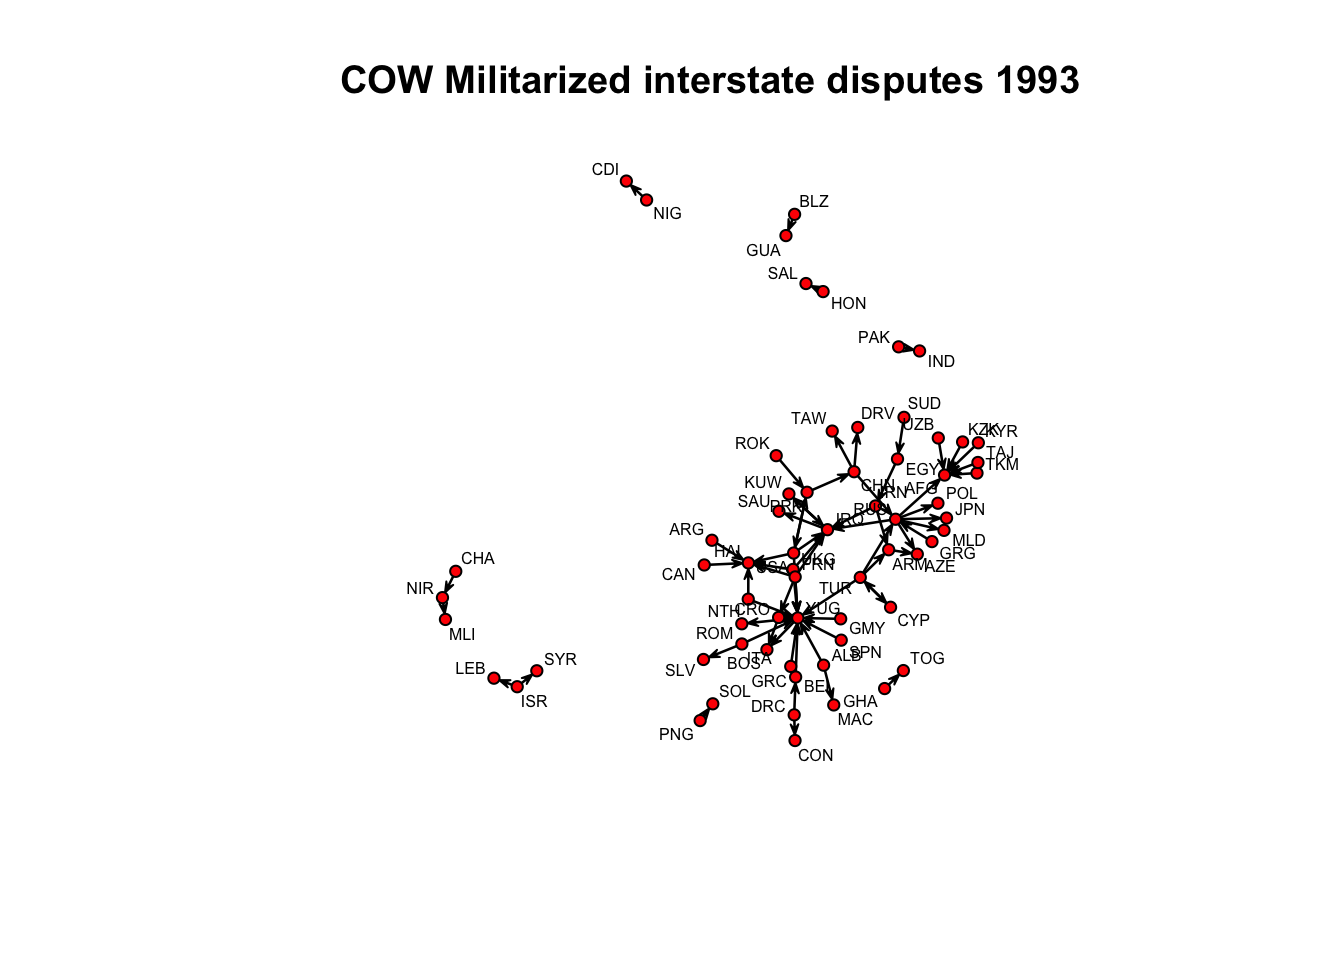
\includegraphics{IntroToNetworks_files/figure-latex/unnamed-chunk-20-1.pdf}

R code

\begin{Shaded}
\begin{Highlighting}[]
\KeywordTok{data}\NormalTok{(emon)}
\NormalTok{imar<-}\KeywordTok{c}\NormalTok{(}\DecValTok{5}\NormalTok{, }\DecValTok{4}\NormalTok{, }\DecValTok{4}\NormalTok{, }\DecValTok{2}\NormalTok{) +}\StringTok{ }\FloatTok{0.1}
\NormalTok{nmar<-.}\DecValTok{75}\NormalTok{*imar}
\KeywordTok{par}\NormalTok{(}\DataTypeTok{mfrow=}\KeywordTok{c}\NormalTok{(}\DecValTok{2}\NormalTok{,}\DecValTok{4}\NormalTok{), }\DataTypeTok{mar=}\NormalTok{nmar)}
\NormalTok{for(i in }\DecValTok{1}\NormalTok{:}\DecValTok{7}\NormalTok{)\{}
  \KeywordTok{plot.network}\NormalTok{(emon[[i]], }\DataTypeTok{usearrows=}\OtherTok{FALSE}\NormalTok{, }\DataTypeTok{vertex.cex=}\FloatTok{1.5}\NormalTok{)}
     \KeywordTok{mtext}\NormalTok{(}\KeywordTok{names}\NormalTok{(emon)[i],}\DataTypeTok{side=}\DecValTok{1}\NormalTok{, }\DataTypeTok{edge.col=}\StringTok{"grey"}\NormalTok{)}
    \NormalTok{\}}
\end{Highlighting}
\end{Shaded}

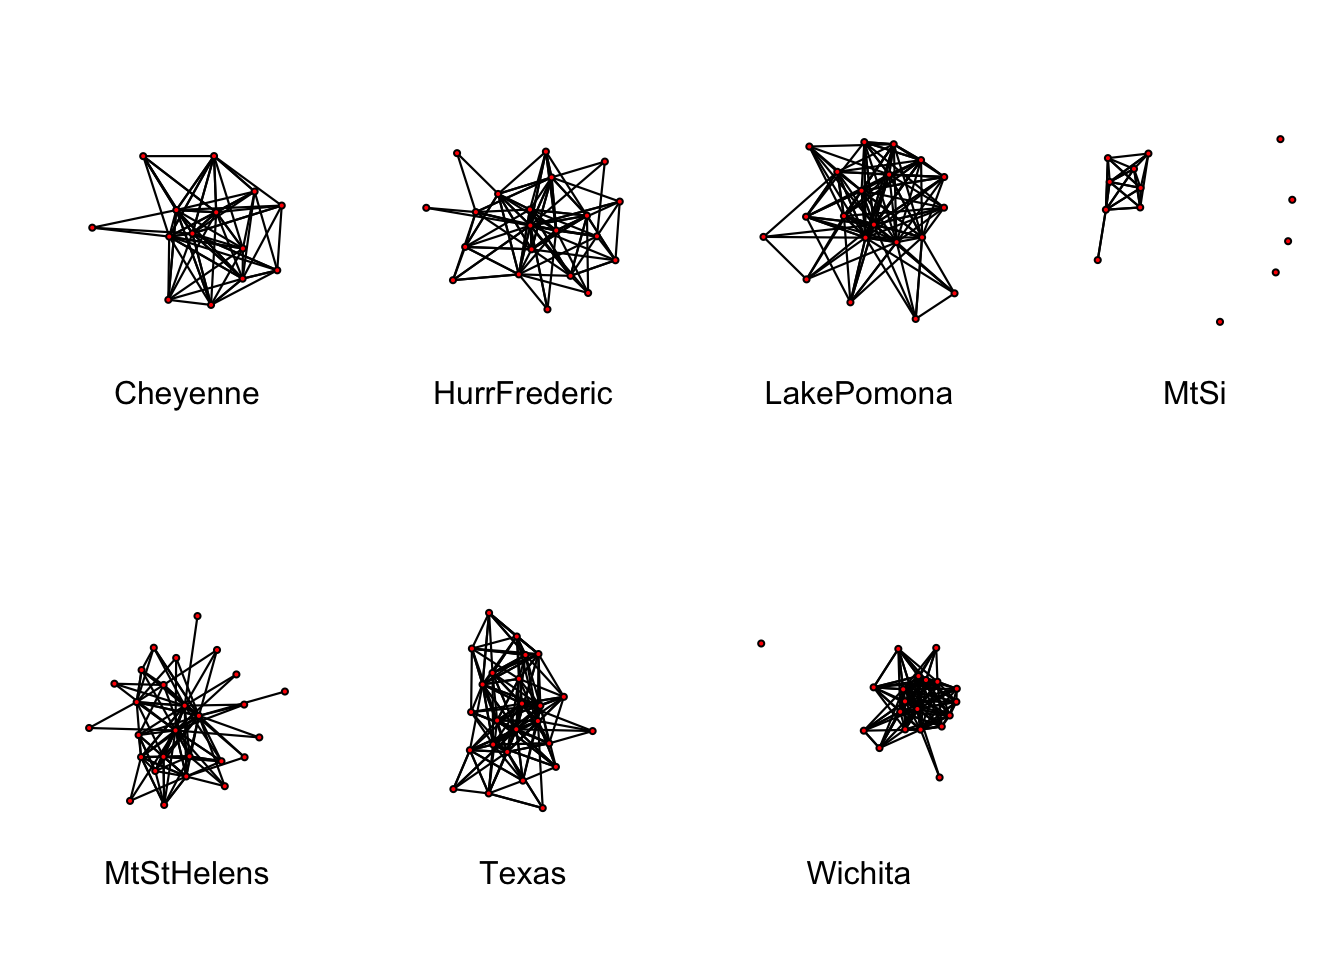
\includegraphics{IntroToNetworks_files/figure-latex/unnamed-chunk-21-1.pdf}

\begin{itemize}
\tightlist
\item
  Interpersonal networks

  \begin{itemize}
  \tightlist
  \item
    Communication - e.g.~WTC responder radio communications (aggregate
    and dynamic
  \item
    Friendship - e.g.~perceived and estimated friendships among managers
  \item
    Interaction in task performance- e.g.~WTC police reports
  \item
    Co-Participation- e.g.~research group co-participation in a large
    research project
  \end{itemize}
\item
  Citation networks

  \begin{itemize}
  \tightlist
  \item
    Authorship- e.g.~authorship of articles in a large research project
  \item
    hyperreferences- e.g.~citations among weblogs
  \item
    Functional Citations- e.g.~function calls in the linux kernel
  \end{itemize}
\item
  Conceptual networks

  \begin{itemize}
  \tightlist
  \item
    Interval graphs- e.g.~life history graphs
  \item
    Mental models- e.g.~student concept maps for ``information systemÓ
  \item
    Entailment structures- e.g.~latent structure in US religious belief;
    dependencies within the Bank Wiring Room
  \end{itemize}
\end{itemize}

A special case of a node not attached to any other vertex is known as an
\textbf{isolate} and will be carefully definee as a component of size 1.
We will discuss this more in the future.

\section{STATNET Overview}\label{statnet-overview}

Using the \emph{network} package to handle \textbf{Network objects}.

Basics in getting and loading a network example data-set:

\begin{Shaded}
\begin{Highlighting}[]
\KeywordTok{library}\NormalTok{(network)       }\CommentTok{# Make sure that network is loaded}
\CommentTok{# help("network-package") to get started.}
\KeywordTok{data}\NormalTok{(}\DataTypeTok{package=}\StringTok{"network"}\NormalTok{) }\CommentTok{# List available datasets in network}

\KeywordTok{data}\NormalTok{(flo)      }\CommentTok{# Load a built-in data set; see ?flo for more}
\NormalTok{flo          }\CommentTok{# Examine the flo adjacency matrix}
\end{Highlighting}
\end{Shaded}

\BeginKnitrBlock{example}
\protect\hypertarget{exm:unnamed-chunk-23}{}{\label{exm:unnamed-chunk-23}
}Common network file types are that of the tables (.txt or .csv), Pajek
network format (\url{http://vlado.fmf.uni-lj.si/pub/networks/pajek/},
UCINET, etc.
\EndKnitrBlock{example}

First find the files ``flo.paj'' and ``floadj.txt'' that come within the
network package:

First we will attempt to bring in a .txt file:

\begin{Shaded}
\begin{Highlighting}[]
 \NormalTok{flo.paj.location <-}\StringTok{"http://vlado.fmf.uni-lj.si/pub/networks/data/GD/gd98/A98.net"}
\end{Highlighting}
\end{Shaded}

Try reading in a Pajek file:

\begin{Shaded}
\begin{Highlighting}[]
\NormalTok{flopaj <-}\StringTok{ }\KeywordTok{read.paj}\NormalTok{(flo.paj.location)}
\end{Highlighting}
\end{Shaded}

Write to table

\begin{Shaded}
\begin{Highlighting}[]
\KeywordTok{write.table}\NormalTok{(flopaj[,],}\DataTypeTok{file=}\StringTok{"data/floadj.txt"}\NormalTok{)}
\NormalTok{floadj.txt.location <-}\StringTok{"data/floadj.txt"}
\end{Highlighting}
\end{Shaded}

Then read them into adjacency matrix form:

\begin{Shaded}
\begin{Highlighting}[]
 \NormalTok{floadj <-}\StringTok{ }\KeywordTok{read.table}\NormalTok{(floadj.txt.location,}\DataTypeTok{header=}\OtherTok{TRUE}\NormalTok{)}
 \NormalTok{floadj  }
\end{Highlighting}
\end{Shaded}

Some other common commands and calls for network class types:

\begin{Shaded}
\begin{Highlighting}[]
\KeywordTok{names}\NormalTok{(flopaj)    }\CommentTok{# This is a project file, with networks and other data}
\KeywordTok{names}\NormalTok{(flopaj$networks)  }\CommentTok{# See which networks are in the file}

\NormalTok{nflo2 <-}\StringTok{ }\NormalTok{flopaj$networks[[}\DecValTok{1}\NormalTok{]]   }\CommentTok{# Extract the marriage data}
\NormalTok{nflo2       }\CommentTok{# Examine the network object}
\end{Highlighting}
\end{Shaded}

Load ``native'' R data file( note, may need to change directory).

\begin{Shaded}
\begin{Highlighting}[]
\KeywordTok{load}\NormalTok{(}\StringTok{"data/nmlec1.Rdata"}\NormalTok{)         }\CommentTok{# Load example data}
\NormalTok{mids_1993            }\CommentTok{# Examine one of the imported objects}
\end{Highlighting}
\end{Shaded}

\BeginKnitrBlock{example}
\protect\hypertarget{exm:unnamed-chunk-30}{}{\label{exm:unnamed-chunk-30} }
Other useful R commands in the network package. As always one can delve
deeper into these functions via R's help manuals (either \emph{?} or
\emph{help()} ).

One of the first things we should look at is network objects, here is a
quick example of how to create a network object and pull out some basic
network properties.
\EndKnitrBlock{example}

\begin{Shaded}
\begin{Highlighting}[]
\KeywordTok{data}\NormalTok{(flo)}
\NormalTok{nflo <-}\StringTok{ }\KeywordTok{network}\NormalTok{(flo, }\DataTypeTok{directed=}\OtherTok{FALSE}\NormalTok{)     }
\NormalTok{nflo   }\CommentTok{# Get a quick description of the data}
\KeywordTok{summary}\NormalTok{(nflo)   }\CommentTok{# Get an overall summary}
\KeywordTok{print}\NormalTok{(nflo)    }\CommentTok{# Simple print method}
\KeywordTok{network.dyadcount}\NormalTok{(nflo)   }\CommentTok{# How many dyads in nflo?}
\KeywordTok{network.edgecount}\NormalTok{(nflo)     }\CommentTok{# How many edges are present?}
\KeywordTok{network.size}\NormalTok{(nflo)   }\CommentTok{# How large is the network?}
\KeywordTok{as.sociomatrix}\NormalTok{(nflo)   }\CommentTok{# Show it as a sociomatrix}
\NormalTok{nflo[,]   }\CommentTok{# Another way to do it}
\end{Highlighting}
\end{Shaded}

An example plot generated by the \emph{plot.network()} command. The plot
on the left is the default Fruchterman and Reingold's force-directed
placement algorithm, where the plot on the right is a circle output.
More layouts and information can be found with \emph{gplot} function.

\begin{Shaded}
\begin{Highlighting}[]
\KeywordTok{par}\NormalTok{(}\DataTypeTok{mfrow=}\KeywordTok{c}\NormalTok{(}\DecValTok{1}\NormalTok{,}\DecValTok{2}\NormalTok{))}
 \KeywordTok{plot}\NormalTok{(nflo,}\DataTypeTok{displaylabels=}\NormalTok{T,}\DataTypeTok{boxed.labels=}\NormalTok{F) }
 \KeywordTok{plot}\NormalTok{(nflo,}\DataTypeTok{displaylabels=}\NormalTok{T,}\DataTypeTok{mode=}\StringTok{"circle"}\NormalTok{, }\DataTypeTok{boxed.labels=}\NormalTok{F) }
\end{Highlighting}
\end{Shaded}

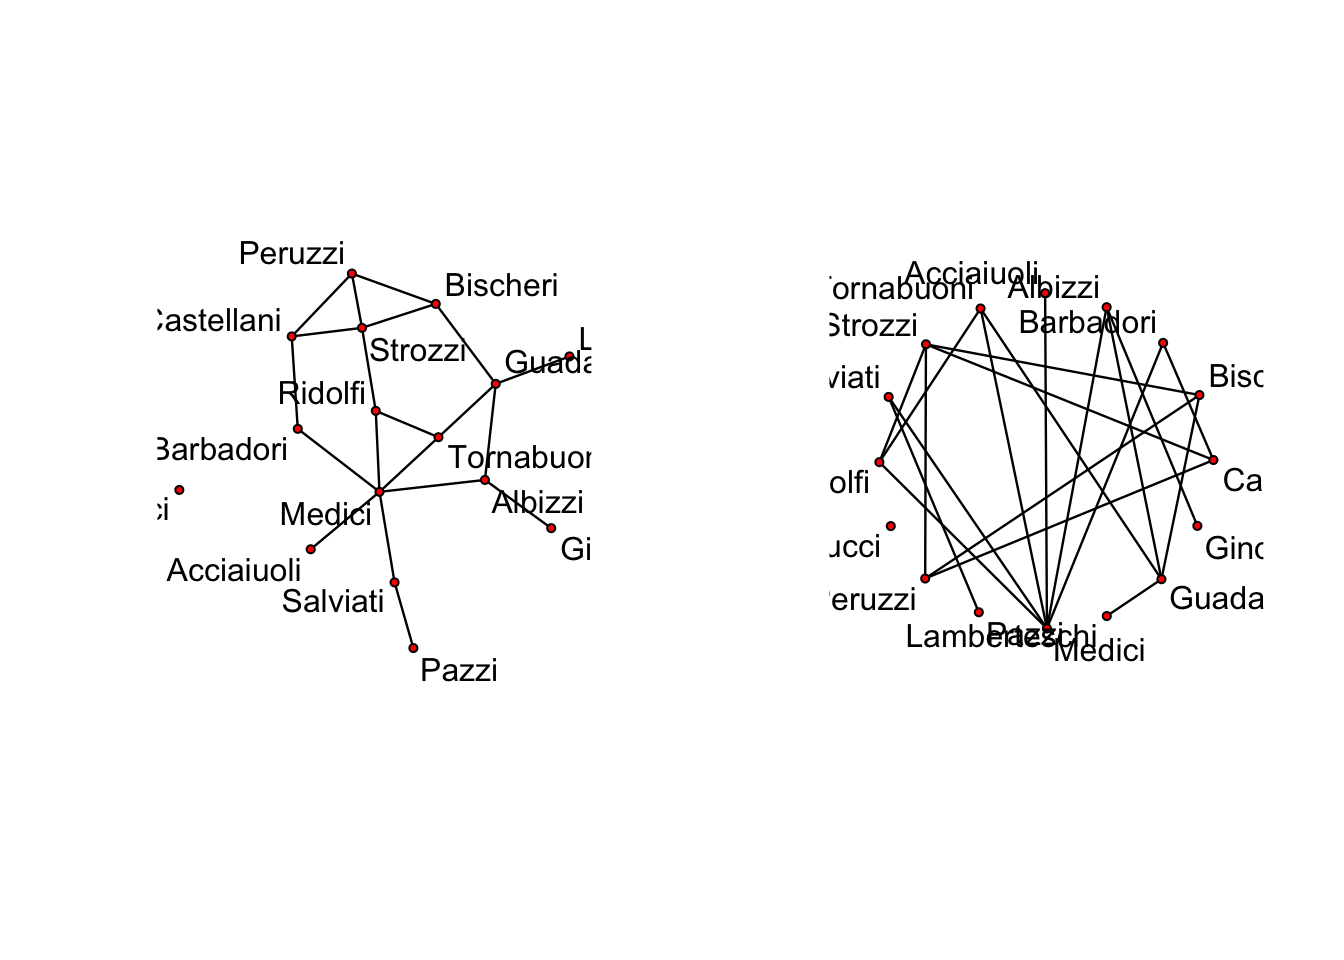
\includegraphics{IntroToNetworks_files/figure-latex/unnamed-chunk-32-1.pdf}

```

Generating an empty network can be useful for a number of things.

\begin{Shaded}
\begin{Highlighting}[]
 \CommentTok{# Create an empty graph with 5 vertices}
\NormalTok{nempty <-}\StringTok{ }\KeywordTok{network.initialize}\NormalTok{(}\DecValTok{5}\NormalTok{) }
\NormalTok{nempty   }\CommentTok{# Compare with nflo  }
\end{Highlighting}
\end{Shaded}

Now, we can look at some basic network properties such as edges.

\begin{Shaded}
\begin{Highlighting}[]
\NormalTok{g <-}\StringTok{ }\KeywordTok{network.initialize}\NormalTok{(}\DecValTok{5}\NormalTok{)  }\CommentTok{# Create an empty graph}
 \NormalTok{g[}\DecValTok{1}\NormalTok{,}\DecValTok{2}\NormalTok{] <-}\StringTok{ }\DecValTok{1} \CommentTok{# Add an edge from 1 to 2}
 \NormalTok{g[}\DecValTok{2}\NormalTok{,] <-}\StringTok{ }\DecValTok{1}   \CommentTok{# Add edges from 2 to everyone else}
 \NormalTok{m <-}\StringTok{ }\KeywordTok{matrix}\NormalTok{(}\DecValTok{0}\NormalTok{, }\DataTypeTok{nrow=}\DecValTok{5}\NormalTok{, }\DataTypeTok{ncol=}\DecValTok{5}\NormalTok{)   }
 \NormalTok{m[}\DecValTok{3}\NormalTok{,}\DecValTok{4}\NormalTok{:}\DecValTok{5}\NormalTok{] <-}\StringTok{ }\DecValTok{1} \CommentTok{# Add entries from 3 to 4 and 5}
 \NormalTok{g[m>}\DecValTok{0}\NormalTok{] <-}\StringTok{ }\DecValTok{1}  \CommentTok{# Add more entries}
 \NormalTok{g[,]}
\end{Highlighting}
\end{Shaded}

Some more useful R tricks with adjancy matrices.

\begin{Shaded}
\begin{Highlighting}[]
\CommentTok{# Delete edges}
 \NormalTok{g[}\DecValTok{3}\NormalTok{,}\DecValTok{5}\NormalTok{] <-}\StringTok{ }\DecValTok{0}   \CommentTok{# Remove the edge from 3 to 5}
 \NormalTok{g[,] <-}\StringTok{ }\DecValTok{0}    \CommentTok{# Remove all edges}
 \CommentTok{#Testing adjacency}
 \NormalTok{nflo[}\DecValTok{9}\NormalTok{,}\DecValTok{3}\NormalTok{]    }\CommentTok{# Medici to Barbadori?}
 \NormalTok{nflo[}\DecValTok{9}\NormalTok{,]       }\CommentTok{# Entire Medici row}
 \NormalTok{nflo[}\DecValTok{1}\NormalTok{:}\DecValTok{4}\NormalTok{,}\DecValTok{5}\NormalTok{:}\DecValTok{8}\NormalTok{]      }\CommentTok{# Subsets are possible}
 \NormalTok{nflo[-}\DecValTok{9}\NormalTok{,-}\DecValTok{9}\NormalTok{]}\CommentTok{# Negative numbers _exclude_ nodes}
 \NormalTok{m <-}\StringTok{ }\KeywordTok{matrix}\NormalTok{(}\DecValTok{1}\NormalTok{:}\DecValTok{16}\NormalTok{^}\DecValTok{2}\NormalTok{, }\DataTypeTok{nrow=}\DecValTok{16}\NormalTok{, }\DataTypeTok{ncol=}\DecValTok{16}\NormalTok{)  }
 \NormalTok{nflo %e%}\StringTok{ "boo"} \NormalTok{<-}\StringTok{ }\NormalTok{m  }\CommentTok{# Value the marriage ties}

 \CommentTok{#Retrieving edge values}
\KeywordTok{list.edge.attributes}\NormalTok{(nflo)  }\CommentTok{# See what's available}
\NormalTok{nflo %e%}\StringTok{ "boo"}   \CommentTok{# Use the %e% operator}
\KeywordTok{as.sociomatrix}\NormalTok{(nflo,}\DataTypeTok{attrname=}\StringTok{"boo"}\NormalTok{) }
\end{Highlighting}
\end{Shaded}

Now, we can look at vertex attributes (these include things like node
level covariates).

\begin{Shaded}
\begin{Highlighting}[]
\CommentTok{#Add some attributes}
 \NormalTok{nflo %v%}\StringTok{ "woo"} \NormalTok{<-}\StringTok{ }\NormalTok{letters[}\DecValTok{1}\NormalTok{:}\DecValTok{16}\NormalTok{]   }
 \NormalTok{nflo %n%}\StringTok{ "zoo"} \NormalTok{<-}\StringTok{ "R is TanFastic!"}   

 \CommentTok{#Listing attributes}
 \KeywordTok{list.vertex.attributes}\NormalTok{(nflo)   }\CommentTok{# List all vertex attributes}
 \KeywordTok{list.network.attributes}\NormalTok{(nflo)  }\CommentTok{# List all network attributes}
 \CommentTok{#Retrieving attributes}
 \NormalTok{nflo %v%}\StringTok{ "woo"}    \CommentTok{# Retrieve the vertex attribute}
 \NormalTok{nflo %n%}\StringTok{ "zoo"}   \CommentTok{# Retrieve the network attribute}
\CommentTok{# ?attribute.methods}
\end{Highlighting}
\end{Shaded}

```

\chapter{Network Vizualization}\label{networkvizualization}

\chapter{Network Data and
Measurement}\label{network-data-and-measurement}

\section{Types of network data}\label{types-of-network-data}

\subsection{One mode data}\label{one-mode-data}

One-mode data is network data with one vertex class and can be
represented as an adjacency matrix. Simple examples include
organizations, individuals, concepts etc.

\subsection{Two mode data}\label{two-mode-data}

\begin{itemize}
\item Networks with two vertex classes
\begin{itemize}
\item Different entity types, membership, matching/containment
\item Bipartite (enforced bipartite graph)
\item Hypergraph representation (hard to draw in most cases)
\end{itemize}
\item Represented by incidence matrices
\begin{itemize}
\item ``senders" on rows, ``receivers" columns
\item vertex by edges, n by m matrix
\item e.g. %%%%%%%%%give an example incidence
\item e.g. %%%%%%%%%hyper graph example
\end{itemize}
\item Can be used to obtain ``dual" representations
\begin{itemize}
\item 
\end{itemize}
\end{itemize}

\subsubsection{One-mode projections}

\index{two-mode data!one-mode projections}

Let A be an \(N \times M\) incidence matrix; the row-projection of A is
the \(N\times N\) matrix B such that
\(B_{ij}=\sum_{k=1}^M A_{ik}A_{jk}\); likewise, the column projection of
A is the \(M\times M\) matrix C such that
\(C_{ij}=\sum_{k=1}^N A_{ki}A_{kj}\)

\noindent
Matrix notation \(B=AA^T\) and \(C=A^TA\).

\begin{definition} \label{projections} \index{projections}
What do \emph{projections} mean? Projections have simple meaning, Row projections ($B_{ij}$): is the number of column elements shared by row elements i and j. Column projections($C_{ij}$): is the number of row elements shared by column elements i and j.
\end{definition}

\begin{example}\label{onemodeproj}
The number of shared interest between two faculty; number of faculty having a given interest area in common.
%%build simple example and add
\end{example}

\subsubsection{Entailments from two-mode data}

\begin{definition} \label{entailment} \index{two-mode data!entailment}
\textbf{Entailment}: relationship of the form ``A implies B."

Inclusion-based entailment:
\begin{itemize}
\item Row: if row entity i is tied to column entity k, so is row entity j
\item Column: if column entity i is tied to row entity k, so is column entity j 
\item From the two-mode data in example \ref{onemodeproj}: faculty who are interested in mathematical sociology are also interested in social networks (but not always vice versa!) 
\item From the two-mode data in example \ref{onemodeproj}: whatever K. Faust is interested in, so is L. Freeman 
\item  Used in analyzing ownership patterns4 
\end{itemize}

\end{definition}

\subsection{Network data collection}

To analyze network data, we must first collect it. Many approaches exist
Ð some better than others for particular purposes, this is a complex
topic overall, but we will at least skim the surface \dots

Two important concepts (not always separable):

\begin{itemize}
\item \underline{Instruments}: tools used to elicit information from 
respondents, assess presence/absence of ties from 
sensors or archival materials, etc. 
\item \underline{Designs}: protocols for determining how information 
should be elicited, who should be sampled, etc.
\end{itemize}

\subsection{Relational Data - Designs}

\textbf{Own-tie reports}

\begin{itemize}
\item Personal ties elicited from each ego 
\item Standard instruments: roster and name generator 
\item Pros: Easily implemented, most common design 
\item Cons: Vulnerable to reporting Relational Data - Designs 
\end{itemize}

\noindent
\textbf{Egocentric network sampling}

\begin{itemize}
\item Personal ties elicited from ego, followed by induced ties 
\item Standard instrument: name generator followed by roster 
\item Pros: Well-suited to large-scale survey sampling; provides information 
on ego's neighborhood 
\item Cons: Vulnerable to reporting error; false positives/negatives on own 
ties contaminate sampling of neighbors' ties Instruments: Name Generators 
and Rosters 
\end{itemize}

\subsection{Instruments}

\subsubsection{Name Generators and Rosters}

\begin{multicols}{2}
\noindent
\textbf{Name generator}: asks 
respondents to list names 
\begin{itemize}
\item E.g. ``Think about the persons 
with whom you have talked in 
the past week.  Please list all 
such persons in the following 
space." (followed by space to 
enter names) 
\end{itemize}

\noindent
Pros: 
\begin{itemize}
\item Don't have to know name list; 
can use with large groups or 
organizations 
\end{itemize}

\noindent
Cons: 
\begin{itemize}
\item High rate of forgetting; unclear 
boundary 
\end{itemize}

\noindent
\textbf{Roster}: asks respondents 
to choose names from 
fixed list 
\begin{itemize}
\item E.g. ``For each of the following 
persons, place a check in the 
associated blank if you have 
talked with him her in the past 
week." (followed by check list) 
\end{itemize}

\noindent
Pros: 
\begin{itemize}
\item More accurate, clear boundary 
\end{itemize}


\noindent
Cons: 
\begin{itemize}
\item List may be prohibitively long, 
can be imposing; alters must 
be known in advance
Instruments: Complete ego-net 
\end{itemize}
\end{multicols}

\subsubsection{Complete ego-net}

Common way to elicit ego nets: complete instrument followed by roster

We have briefly mentioned this form of data collecting before. One is
asked to name those with whom you discussed important matters Then,
asked to fill in same question for all pairs of persons named initially
(see \textbf{Problem} \ref{lec12:prob1}). Pros: Relatively easy to
administer; don't need entire list of possible alters; don't have to ask
about all group members. Cons: Step 1, step 2 questions have different
error rates; may need large roster if many alters; hard to use with
paper-based surveys

\subsubsection{Coding Schemes as ``instruments" }

Can also think of coding schemes for archival materials as
``instruments"

\begin{example}\label{csinst} of Coding Schemes as ``instruments."


\begin{itemize}
\item Transcripts \\

Tag each line by sender/receiver; (i,j) tie if i sends to j.\\

\item Descriptive lists/tables \\

Common for two-mode data. Build entity/property table; fill in (i,j) as 1 if ith row entity has 
property j.\\ 
 
\item Video/Audio \\

Determine criterion for interaction. Find all interactions, code by sender/receiver; (i,j) tie if i sends to j.\\ 
 
\item Narrative documents \\

Determine criterion for interactions. As before, code by sender/receiver (or just by dyad, if not directed)  (i,j) tie if i sends to j, or \{i,j\} tie if i and j interact.
\end{itemize}
\end{example}

\subsection{Designs}

\begin{itemize} 
\item Own-tie reports 
\begin{itemize}
\item Personal ties elicited from each ego 
\item Standard instruments: roster and name generator 
\item Pros: Easily implemented, most common design 
\item Cons: Vulnerable to reporting error 
\end{itemize}
\item Egocentric network sampling 
\begin{itemize}
\item Personal ties elicited from ego, followed by induced ties 
\item Standard instrument: name generator followed by roster 
\item Pros: Well-suited to large-scale survey sampling; provides information 
on ego's neighborhood 
\item Cons: Vulnerable to reporting error; false positives/negatives on own 
ties contaminate sampling of neighbors' ties
\end{itemize}
\item Link-tracing 
\begin{itemize}
\item Personal ties elicited from ego; new ego(s) chosen from alters; process is iterated 
(possibly many times) 
\item Standard instruments: multiwave own-report, RDS 
\item Pros: Allows estimation of network properties for large and/or hard to reach 
populations; highly scalable; can be robust to poor seed sampling 
\item Cons: Vulnerable to reporting error; reporting errors can contaminate design (but may 
be less damaging than ego net case); often difficult to execute 
\end{itemize}
\item Arc-sampling 
\begin{itemize}
\item Reports on third-party ties elicited from ego; multiple egos may be sampled for each 
third-party tie 

\indent Archival/observer data is a special case 

\item Standard instrument: CSS 
\item Pros: Very robust to reporting error (via modeling); can be very robust to missing data 
\item Cons: Can impose large burden on respondents; can be difficult to execute
\end{itemize}
\end{itemize}

\subsection{Designs: CSS and RDS}\begin{multicols}{2}
\noindent
\textbf{Cognitive Social Structure (CSS)}
\begin{itemize} 
\item Ask each group member to 
report on all members' ties 
\item Ex: "Which of the following 
persons does Steve go to for 
help or advice?" 
\end{itemize}

\noindent
\textbf{Pros:}
\begin{itemize} 
\item Gets information on 
perception; can be used to get 
high-accurate estimates 
\end{itemize}

\noindent
\textbf{Cons:}
\begin{itemize} 
\item Hard to use; requires roster; 
doesn't scale well 
\end{itemize}

\noindent
\textbf{Respondent Driven Sampling (RDS) }
\begin{itemize}
\item Combine standard network 
instrument with recruitment 
"tickets" 
\item Respondents given tickets to 
give to others; if they 
volunteer, both get paid 
\end{itemize}

\noindent
\textbf{Pros:}
\begin{itemize} 
\item Can use with hidden, 
vulnerable populations 
\end{itemize}

\textbf{Cons:} 
\begin{itemize}
\item Difficult; expensive; complex 
to analyze; poorly understood
\end{itemize}
\end{multicols}

\subsection{Network Boundary Problems}

How do we define the node or vertex set? If misspecified, theoretically
relevant ties may be missed.

\textbf{Typical cases}

\begin{itemize} 
\item Exogenously defined-- Physical region, group/cohort membership 
 \item Relationally defined-- Isolated social unit (component), locally dense 
 \item Design defined-- Alters named in ego net, link trace; sampled egos 
\end{itemize}

\noindent
 \textbf{Notes} Major distinction: local versus global properties.
Different sampling methods needed for each.

\chapter{Network Descriptive
Statistics}\label{network-descriptive-statistics}

\bibliography{book.bib,packages.bib,snatextbib.bib}


\end{document}
